\documentclass[a4paper]{article}
\def\DOCTITLE{CSC3223 Graphics for Games}
% Set document attributes
\title{\DOCTITLE}

\usepackage{fullpage}
\usepackage{scrextend}
\usepackage{titlesec}
\usepackage{fancyhdr}
\usepackage{amsmath}
\usepackage{amssymb}
\usepackage[section]{placeins}
\usepackage{booktabs}
\usepackage{hyperref}
\usepackage{tikz}
\usepackage{graphicx}
\usepackage{minted}
\usepackage{subcaption}

% Setup headers and footers
\pagestyle{fancy}
\lhead{}
\chead{\DOCTITLE}
\rhead{}
\rfoot{}
\cfoot{\thepage}
\lfoot{}

% New page for each section
\newcommand{\sectionbreak}{\clearpage}

% Set header and footer sizes
\renewcommand{\headrulewidth}{0.4pt}
\renewcommand{\footrulewidth}{0.4pt}
\setlength{\headheight}{15.2pt}
\setlength{\headsep}{15.2pt}

\setlength{\parskip}{5pt plus 1pt minus 1pt}
\setlength{\parindent}{0pt}

% Newline after paragraph
\newcommand{\Para}[1]{\paragraph{#1}\mbox{}}

% Stuff used in cryptography notes
\newcommand{\Forall}{\;\forall\;}
\newcommand{\Mod}{\: mod \:}

% Stuff used in distributed systems notes
\newcommand{\happenbefore}{\rightarrow}
\newcommand{\orderbefore}{\Rightarrow}
\newcommand{\clockcond}{\leadsto}
\newcommand{\RArrow}{$\rightarrow$}

\def\checkmark{\tikz\fill[scale=0.4](0,.35) -- (.25,0) -- (1,.7) -- (.25,.15) -- cycle;}


\begin{document}

\tableofcontents

\section{Overview}

\subsection{3D Graphics}

\begin{itemize}
  \item Scene made up of objects made up of primitives
  \item Primitives are a collection of vertices
  \item Vertices have attributes (position, colour, texture coordinate, etc.)
\end{itemize}

\subsubsection{Primitives}

\begin{figure}[h]
  \centering

  \begin{subfigure}[b]{0.3\textwidth}
    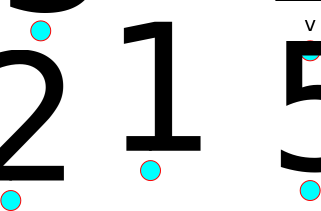
\includegraphics[width=0.8\textwidth]{out/rast_pri_points.eps}
    \caption{Point}
  \end{subfigure}
  \begin{subfigure}[b]{0.3\textwidth}
    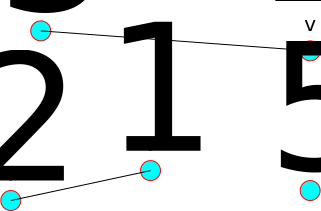
\includegraphics[width=0.8\textwidth]{out/rast_pri_lines.eps}
    \caption{Line}
  \end{subfigure}
  \begin{subfigure}[b]{0.3\textwidth}
    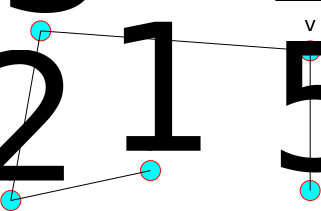
\includegraphics[width=0.8\textwidth]{out/rast_pri_line_strip.eps}
    \caption{Line Strip}
  \end{subfigure}

  \vspace{2em}

  \begin{subfigure}[b]{0.3\textwidth}
    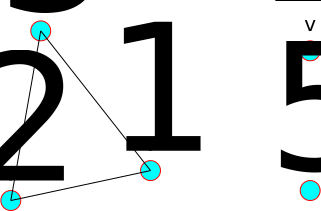
\includegraphics[width=0.8\textwidth]{out/rast_pri_triangle.eps}
    \caption{Triangle}
  \end{subfigure}
  \begin{subfigure}[b]{0.3\textwidth}
    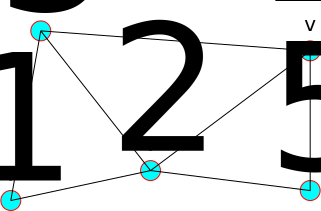
\includegraphics[width=0.8\textwidth]{out/rast_pri_triangle_strip.eps}
    \caption{Triangle Strip}
  \end{subfigure}
  \begin{subfigure}[b]{0.3\textwidth}
    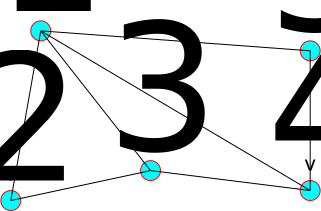
\includegraphics[width=0.8\textwidth]{out/rast_pri_triangle_fan.eps}
    \caption{Triangle Fan}
  \end{subfigure}

  \caption{}
  \label{fig:primitives}
\end{figure}
\FloatBarrier

\subsection{Graphics Pipeline}

\begin{figure}[h!]
  \centering
  \includegraphics[width=0.6\textwidth]{out/graphic_pipeline.eps}
  \caption{Pipeline}
  \label{fig:graphics_pipeline}
\end{figure}
\FloatBarrier

\subsubsection{Vertex Operations}

\begin{enumerate}
  \item[1] Vertices are transformed through a number of matrix operations
           (section \ref{sec:transformations})
  \item[2] Primitives outside screen space are removed (culled)
  \item[3] Vertices outside the screen space are clipped
  \item[4] 3D scene is projected onto a 2D plane
\end{enumerate}

\subsubsection{Fragment Operations}

\begin{enumerate}
  \item[1] Once screen area for a primitive is determined it is rasterised
           (section \ref{sec:rasterisation})
  \item[2] Each fragment is then shaded depending on colour, texture, lighting,
           etc.
\end{enumerate}

\section{Rasterisation}
\label{sec:rasterisation}

\subsection{Line}

Rasterise using Bresenham's line algorithm.

Very simple and fast algorithm for rasterising a line given two 2D points
$(x_{0}, y_{0})$ and $(x_{1}, y_{1})$.

\begin{enumerate}
  \item[1]
    Determine if the line is steep or shallow with respect to the $x$ axis \\
    A steep line is closer being parallel with the $y$ axis

  \item[2]
    Calculate gradient $m = \delta y / \delta x = (y_{1} - y_{0}) / (x_{1} -
    x_{0})$

  \item[3]
    Iterate over the scan (longer) axis \\
    Maintain coordinates of current pixel and $error$ variable

    \begin{enumerate}
      \item[i]
        Shade pixel at current coordinates

      \item[ii]
        Increment the scan axis of current coordinate

      \item[iii]
        $error = error + m$

      \item[iv]
        If $error \geq 0.5$ then increment the periodic axis of current coordinate
        and set $error = error - 1$

    \end{enumerate}

\end{enumerate}

\subsection{Triangle}

\begin{enumerate}
  \item[1] Compute bounding box around triangle
  \item[2] Iterate through each pixel of each line
  \item[3] If the pixel is inside the triangle then shade it
\end{enumerate}

Two common methods for determining if a point is inside a triangle.

Both based on the creation of a temporary vertex $p$ with coordinates of the
pixel being tested.

\subsubsection{Line Equation method}

\begin{enumerate}
  \item[1] Extend lines out from $p$ to each edge of the triangle that are
           perpendicular to the edge
  \item[2] When the direction of each line is towards $p$, $p$ is inside the
           triangle if the distance of each line is positive
\end{enumerate}

\begin{figure}[h]
  \centering
  \begin{subfigure}[b]{0.48\textwidth}
    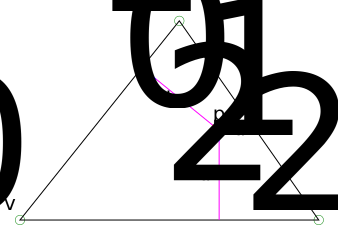
\includegraphics[width=0.8\textwidth]{out/tri_lineeq_in.eps}
    \caption{Inside triangle}
  \end{subfigure}
  \begin{subfigure}[b]{0.48\textwidth}
    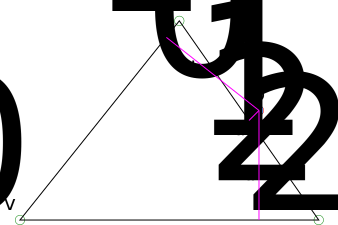
\includegraphics[width=0.8\textwidth]{out/tri_lineeq_out.eps}
    \caption{Outside triangle ($d_{1} < 0$)}
  \end{subfigure}
  \caption{}
  \label{fig:tri_lineeq}
\end{figure}
\FloatBarrier

\subsubsection{Barycentric Coordinate method}
\label{sec:barycentric}

\begin{enumerate}
  \item[1] Create three new triangles ($t_{0}$, $t_{1}$ and $t_{2}$) using $p$
           and vertices of triangle
  \item[2] Calculate area of sub triangles as a proportion of the area of the
           original triangle (using shoelace formula)
  \item[3] If sum of areas of sub triangles $\sum_{i} t_{i} = 1$ then $p$ is
           inside triangle
\end{enumerate}

\begin{figure}[h]
  \centering
  \begin{subfigure}[b]{0.48\textwidth}
    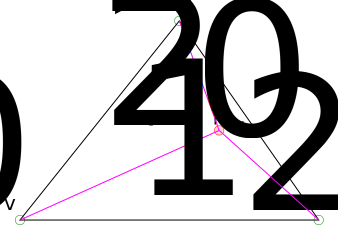
\includegraphics[width=0.8\textwidth]{out/tri_bary_in.eps}
    \caption{Inside triangle}
  \end{subfigure}
  \begin{subfigure}[b]{0.48\textwidth}
    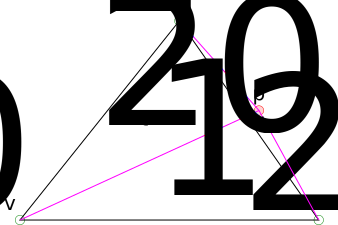
\includegraphics[width=0.8\textwidth]{out/tri_bary_out.eps}
    \caption{Outside triangle}
  \end{subfigure}
  \caption{}
  \label{fig:tri_bary}
\end{figure}
\FloatBarrier

Barycentric areas typically denoted as $\alpha$, $\beta$ and $\gamma$.

\subsubsection{Shoelace formula}

Method of calculating area of any 2D non self-intersecting polygon.

\begin{enumerate}
  \item[1] Create a matrix of the vertices in a closed loop
  \item[2] Multiply the first set of stepped pairs ($s_{1}$)
  \item[3] Multiply the second set of stepped pairs ($s_{2}$)
  \item[4] Calculate area $a = (s_{1}- s_{2}) / 2$
\end{enumerate}

\begin{figure}[h!]
  \centering
  
\includegraphics[width=0.6\textwidth]{graphics/shoelace_formula.eps}
  \caption{Shoelace formula example}
  \label{fig:shoelace_formula}
\end{figure}
\FloatBarrier

\subsubsection{Triangle spans}

Triangles can also be rendered using spans, where it is made up of several
lines.

Span start and end points are obtained using the lines between vertices $v_{0}$
and $v_{1}$ (start) and $v_{2}$ and $v_{1}$ (end).

\begin{figure}[h!]
  \centering
  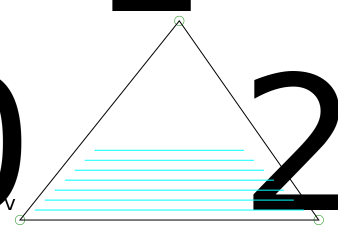
\includegraphics[width=0.6\textwidth]{out/tri_spans.eps}
  \caption{Triangle spans}
  \label{fig:tri_spans}
\end{figure}
\FloatBarrier

\section{Transformations}
\label{sec:transformations}

\subsection{Spaces}

\begin{description}
  \item[World] \hfill \\
    3D space containing everything

  \item[Camera] \hfill \\
    3D space containing the view from the camera \\
    Origin is camera position \\
    Obtained through camera transform

  \item[Clip] \hfill \\
    Only the primitives that can be seen by the camera \\
    Obtained through perspective transform

  \item[Normalised Device Coordinates] \hfill \\
    Transformed from clip space \\
    Coordinates normalised to 1 for hardware compatibility

  \item[Viewport Coordinates] \hfill \\
    Coordinates on a particular screen

\end{description}

\subsection{Scale}

Scale matrix to scale by $x$, $y$ and $z$ is each respective axis:
\[
  \left [
    \begin{array}{cccc}
      x & 0 & 0 & 0 \\
      0 & y & 0 & 0 \\
      0 & 0 & z & 0 \\
      0 & 0 & 0 & 1
    \end{array}
  \right ]
\]

\subsection{Translation}

Translation matrix to move by $x$, $y$ and $z$ is each respective axis:
\[
  \left [
    \begin{array}{cccc}
      1 & 0 & 0 & x \\
      0 & 1 & 0 & y \\
      0 & 0 & 1 & z \\
      0 & 0 & 0 & 1
    \end{array}
  \right ]
\]

\subsection{Rotation}

Rotation about $x$ axis by $\theta$:
\[
  \left [
    \begin{array}{cccc}
      1 & 0           & 0         & 0 \\
      0 & cos\theta   & sin\theta & 0 \\
      0 & -sin\theta  & cos\theta & 0 \\
      0 & 0           & 0         & 1
    \end{array}
  \right ]
\]

Rotation about $y$ axis by $\theta$:
\[
  \left [
    \begin{array}{cccc}
      cos\theta   & 0 & sin\theta & 0 \\
      0           & 1 & 0         & 0 \\
      -sin\theta  & 0 & cos\theta & 0 \\
      0           & 0 & 0         & 1
    \end{array}
  \right ]
\]

Rotation about $z$ axis by $\theta$:
\[
  \left [
    \begin{array}{cccc}
      cos\theta   & sin\theta & 0 & 0 \\
      -sin\theta  & cos\theta & 0 & 0 \\
      0           & 0         & 1 & 0 \\
      0           & 0         & 0 & 1
    \end{array}
  \right ]
\]

\subsection{Perspective}

Perspective matrix used to give perspective to camera space.

\begin{figure}[h!]
  \centering
  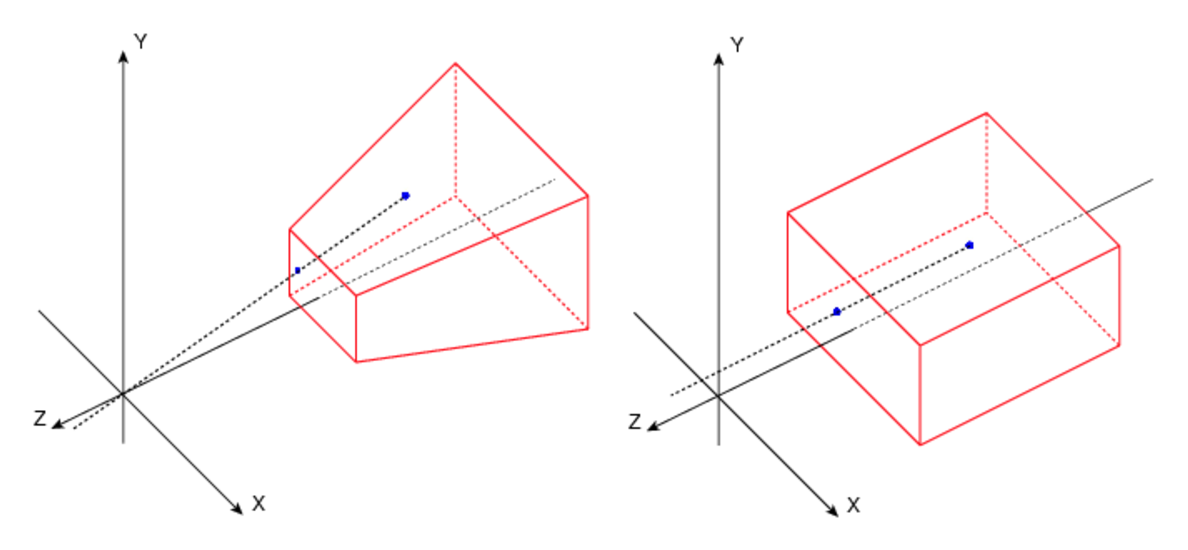
\includegraphics[width=0.6\textwidth]{graphics/perspective-orthographic.eps}
  \caption{Perspective (left) vs Orthographic (right)}
  \label{fig:perspective-orthographic}
\end{figure}
\FloatBarrier

\subsubsection{Orthographic}

Simple clip to a defined box defined by vertices $(left, bottom near)$ and
$(right, top, far)$.
\[
  P =
  \left [
    \begin{array}{cccc}
      \frac{2}{right - left}  & 0                       & 0                     & -\frac{right + left}{right - left} \\
      0                       & \frac{2}{top - bottom}  & 0                     & -\frac{top + bottom}{top - bottom} \\
      0                       & 0                       & \frac{2}{far - near}  & -\frac{far + near}{far - near} \\
      0                       & 0                       & 0                     & 1
    \end{array}
  \right ]
\]

Typically used for "flat" elements, e.g. menu, HUD, etc.

\subsubsection{Perspective}

Traditional perspective as perceived in real life.

\[
  P =
  \left [
    \begin{array}{cccc}
      \frac{f}{aspect}  & 0 & 0                             & 0 \\
      0                 & f & 0                             & 0 \\
      0                 & 0 & \frac{near + far}{near - far} & \frac{2 \cdot near \cdot far}{near - far} \\
      0                 & 0 & -1                            & 0
    \end{array}
  \right ]
\]

where:
\[
  f = \frac{1}{tan(fov / 2)}
\]

and $fov$ is the desired field of view.

\begin{description}
  \item[$x$ and $y$] \hfill \\
    Used to obtain distance along $x$ and $y$ axis with relation to $z$ and
    $fov$

  \item[$z$] \hfill \\
    Scale and translate $z$ position such that $z$ is in the range -1 to 1 after
    division by $w$

  \item[$w$] \hfill \\
    Set to $w = -1 \cdot z = -z$, this is used for the perspective divide

\end{description}

\subsubsection{Perspective Divide}

Have a vector $V$ for a vertex:
\[
  V =
  \left [
    \begin{array}{c}
      V_{x} \\
      V_{y} \\
      V_{z} \\
      w
    \end{array}
  \right ]
\]

Divide components of $V$ by $w$. This operation moves objects that are further
away (in $z$ axis) closer to the centre of the screen, this gives the effect of
a vanishing point.

\subsection{Object definition}

\[
  \left [
    \begin{array}{cccc}
      r_{xx}  & r_{xy}  & r_{xz}  & x \\
      r_{yx}  & r_{yy}  & r_{yz}  & y \\
      r_{zx}  & r_{zy}  & r_{zz}  & z \\
      0       & 0       & 0       & 1
    \end{array}
  \right ]
  \left [
    \begin{array}{c}
      V_{x} \\
      V_{y} \\
      V_{z} \\
      1
    \end{array}
  \right ]
\]

$(x, y, z)$ is the object position.

$r$ is the object orientation.

$(r_{xx}, r_{xy}, r_{xz})$ is the object left vector.

$(r_{yx}, r_{yy}, r_{yz})$ is the object up vector.

$(r_{zx}, r_{zy}, r_{zz})$ is the object facing vector.

The vertices of the object $V$ are transformed using the object matrix.

\subsection{MVP matrix}

Three stages of the standard transformation pipeline:

\begin{description}
  \item[Model] \hfill \\
    Local space to the world space

  \item[View] \hfill \\
    World space to camera space

  \item[Projection] \hfill \\
    Camera space to clip space

\end{description}

\section{Fragment Operations}
\label{sec:fragment_operations}

\subsection{Interpolation}

\Para{Lines}

Colour at point $p$ computed through simple linear interpolation between
vertices $v_{0}$ and $v_{1}$.
\begin{align*}
  C_{p} &= (C_{b} * t) + (C_{a} * (1 - t)) \\
      t &= |(v_{1} - p) / (v_{1} - v_{0})|
\end{align*}

\Para{Triangles}

Use Barycentric coordinates (section \ref{sec:barycentric}).
\[
  C_{p} = (\alpha * C_{a}) + (\beta * C_{b}) + (\gamma * C_{c})
\]

\subsection{Transparency}

Transparency denoted by alpha value in colour.

$\alpha = 1$ denotes full opacity, $\alpha = 0$ denotes full transparency.

Colour computed by blend equation:
\[
  C = (C_{source} * F_{source}) + (C_{dest} * F_{dest})
\]

Factors $F_{source}$ and $F_{dest}$ are usually programmable but a common
approach is standard linear blending:
\begin{align*}
  F_{source} &= \alpha \\
    F_{dest} &= 1 - \alpha
\end{align*}

One other alternative is additive blending:
\begin{align*}
  F_{source} &= 1 \\
    F_{dest} &= 1
\end{align*}

\subsection{Depth Buffer / Depth Test}

Have a depth buffer which records the depth ($z$ coordinate) of the fragment
that has been rendered on a each pixel.

\begin{enumerate}
  \item[1]   When a pixel is to be shaded compare the $z$ coordinate of the new
             fragment with that in the depth buffer $D_{i}$
  \item[2.1] If $x \leq D_{i}$ then depth test passes, the pixel is shaded based
             on the new fragment and the depth buffer updated
  \item[2.1] Otherwise the test fails and the fragment is discarded
  \item[3]   The depth buffer is rest to maximum depth at the start of each
             frame
\end{enumerate}

Can have "z fighting" when two objects with close $z$ coordinates are rasterised
inside each other. A higher precision depth buffer avoids this.

\section{Texture Mapping}

\begin{itemize}
  \item Texture coordinates $(u, v)$ defined per vertex
  \item Coordinated interpolated to obtain per fragment texture coordinates
  \item $(u, v)$ are normalised texture coordinates within $[0, 1]$
  \item Textures coordinates out of the $[0, 1]$ can be handled differently:
    \begin{description}
      \item[Clamp] \hfill \\
        Anything above 1 is set to 1 \\
        Anything below 0 is set to 0
      \item[Repeat] \hfill \\
        $1.1 = 0.1$ \\
        $-0.1 = 0.9$ \\
        etc.
      \item[Mirror] \hfill \\
        $1.1 = 0.9$ \\
        $-0.1 = 0.1$ \\
        etc.
    \end{description}
  \item All textures for a mesh typically stored in a single texture image
\end{itemize}

\subsection{Affine Transform}

Textures may not appear correctly if an object is tilted with respect to the
camera.

Caused by texture interpolation being linear but not fragment area.

Solution is to use affine transform:

\begin{enumerate}
  \item[1] Divide texture coordinates by $P_{w}$
  \item[2] Interpolate texture coordinates
  \item[3] Multiply by $P_{w}$
\end{enumerate}

\subsection{Bilinear Filtering}

When a texture is viewed close enough to the camera such that the rasterised
object takes up more pixel space than the texture image.

Sample multiple texels and blend them together.

e.g. for texel coordinate 7.6 blend colour of texel 7 and 8 by factor 0.6.

\subsection{MIP mapping /  minification}

Generating smaller textures using the original fill size texture so that objects
further away can sample a smaller texture.

Forms a set of textures in decrecing size, known as a MIP chain.

MIP map is selected using the level of detail (LOD) $\lambda$.

This is calculated using the derivatives of the interpolated $x$ and $y$
texture coordinates, i.e. how fast the texture coordinates are changing.

Faster change in texture coordinates (higher $\lambda$) means less unique texels
hence less detail. The size of $\lambda$ denotes how far down the MIP change the
texture is selected.

MIP chain is pre processed when the texture is loaded.

Requires more memory to store entire MIP chain opposed to a single texture, but
gives faster processing as less work needs to be done during rasterisation and
gives a better texture quality due to texel averaging.

\subsubsection{Trilinear filtering}

Similar to bilinear filtering (operating in $x$ and $y$ axes) but also operating
in $z$ axis to interpolate between two MIP map levels.

Solves issue when an object spans multiple MIP levels and a noticeable line where
the texture quality changes can be seen.

\section{OpenGL}

\begin{figure}[h!]
  \centering
  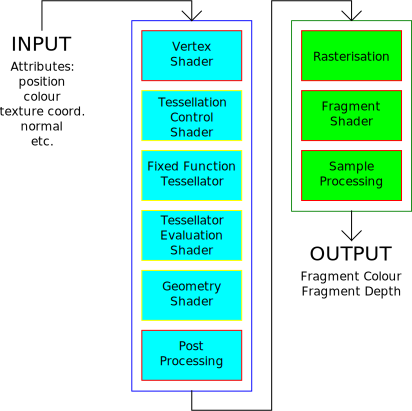
\includegraphics[width=0.8\textwidth]{out/opengl_pipeline.eps}
  \caption{OpenGL Pipeline}
  \label{fig:opengl_pipeline}
\end{figure}
\FloatBarrier

Vertex post processing operations:

\begin{itemize}
  \item Vertex clipping
  \item Perspective divide
  \item Viewport transform
\end{itemize}

Sample processing operations:

\begin{itemize}
  \item Depth test
  \item Alpha blending
\end{itemize}

Note that tessellation shaders, the tessellator, and geometry shaders are
optional.

\subsection{Shaders}

\begin{description}
  \item[Attributes] \hfill \\
    Values specific to the vertex or fragment being processed
  \item[Uniforms] \hfill \\
    Constant for all shader executions
  \item[Interface block] \hfill \\
    Used to interface shaders to each other, e.g. vertex shader $\rightarrow$
    fragment shader
\end{description}

Automatic interpolation between shaders (e.g. values in output block of
vertex/geometry shaders get interpolated before the fragment shader) (can be
disabled using \texttt{flat} layout qualifier).

Textures accessed from any shader through samplers. Textures are bound to a
texture unit which maps to texturing hardware.

\subsection{Geometry Shader}

Used to create new primitives from those created by the CPU side code.

\begin{itemize}
  \item Invoked once per primitive
  \item Input is array of vertices
  \item Output is a number of new primitives
\end{itemize}

Usage examples:

\begin{itemize}
  \item Normal visualisation
  \item Particle systems
\end{itemize}

Reduces processing to be done by the CPU and earlier stages of the pipeline by
reducing the number of vertices they need to process.

Limited number of output vertices (based on specific hardware).

\subsection{Tessellation}

\begin{itemize}
  \item Used for larger scale geometry amplification
  \item Tessellation used to "fill" an existing primitive with more primitives
  \item More vertices generated which can be transformed
\end{itemize}

The hardware tessellator operates on patches (areas bound by a number of
vertices) and turns them in to wither lines, triangles or quads.

Instead of a position, output vertices have a weighting which specifies its
position relative to a number of the input vertices.

Patches have tessellation factors that define how many new new vertices are
generated. One factor for the inside of the patch and several for the outside.

Using these factors it is possible to correctly line up patches with differing
tessellation levels without having "cracks" in the object.

\subsubsection{Tessellation Control Shader}

Invoked once per input patch vertex.

Feeds vertex information to tessellator and controls tessellation levels.

\subsubsection{Tessellation Evaluation Shader}

Invoked for every new vertex.

Converts barycentric weightings created by the tessellator into positions.

\section{Scene Hierarchy and Skeletal animation}

\subsection{Scene Graphs}

\begin{itemize}
  \item Hierarchical tree structure of meshes
  \item Each mesh has a model matrix that gets applied to it and all its
        children
  \item Typically use a tree as shallow as possible to reduce traversal time
  \item Can include many other (non graphical) objects on the tree:
    \begin{itemize}
      \item Sound emitters
      \item Shaders
      \item etc.
    \end{itemize}
\end{itemize}

Need to ensure transparent objects are drawn in the correct order. Solution is
to add a "transparency" tag to each node.

When processing objects:
\begin{enumerate}
  \item[1] Traverse the tree and build a list of opaque objects and a list of
           transparent objects
  \item[2] Render all the opaque objects
  \item[3] Sort the list of transparent objects by their $z$ position
  \item[4] Render transparent object from furthest away to closest
\end{enumerate}

\subsection{Animation}

Can do simple animation by manipulating a tree of objects and their model
matrices. This works well for simple objects such as cars and robots.

It will not work for objects that have a flexible skin (such as humans).

\subsubsection{Skinned meshes}

Instead a skinned mesh is used and each vertex is pulled in the direction of
several skeletal nodes (joints) by a set of weights.

Skeletal nodes are arranged in a hierarchical tree and inherit transformations.

Skinning (the process of transforming vertices of the mesh based on weights) is
typically done on the vertex shader. An array of transformations can be passed
to the shader through a uniform.

The assignment of weights to each vertex and node (rigging) is done offline in
the 3D modelling suite.

In order to get a good frame rate in a skeletal animation without having to
reskin the mesh every frame animation can be interpolated.

In order to combine multiple animations that affect different parts of the
skeleton, different animations can be blended together to form a new animation.

Joints can usually be queried to obtain the transformation, useful when
attaching other meshes to them (e.g. attach a gun to a hand).

Inverse kinematics can be used to position a child node in a given position and
have the parent nodes move in a realistic manner (e.g. placing a hand on a door
handle).

\section{Lighting}

\subsection{Normals}

\begin{itemize}
  \item Unit vector perpendicular to the surface
  \item Can be calculated using cross product of two side vectors
  \item Usually stored as part of the model
  \item Vertex normals are interpolated across the primitive
  \item Interpolation may cause problems if an object has sharp corners
\end{itemize}

\subsection{Lighting Models}

\begin{description}
  \item[Static lighting] \hfill \\
    Combining texture with a light map. \\
    No real time updates. \\
    No additional computation.

  \item[Flat shading] \hfill \\
    Per surface lighting. \\
    No interpolation over surface. \\
    Computationally fast.

  \item[Gourard shading] \hfill \\
    Per vertex shading. \\
    Normal interpolated across primitive. \\
    More computationally expensive.

  \item[Phong shading] \hfill \\
    Per fragment lighting. \\
    Normal interpolated across primitive. \\
    Most computationally intensive.

  \item[Bump Mapping] \hfill \\
    Normals stored in texture. \\
    Each texel has its own normal.

\end{description}

\subsection{Phong Reflection Model}

Types of light:

\begin{description}
  \item[Ambient] \hfill \\
    Lights all faces of all objects in a scene equally
  \item[Diffuse] \hfill \\
    Light from a source that has been scattered evenly
  \item[Specular] \hfill \\
    Light from a source that has been reflected towards the camera
\end{description}

Lighting colour $c$ of a fragment (for a single light):
\begin{align*}
      c &= c_{a} + (c_{d} + c_{s}) \times a \\
  c_{d} &= (N \cdot |(L - P)|) \times C_{d} \\
  c_{s} &= (N \cdot \frac{1}{2}(V + L))^{n} \times C_{s}\\
      a &= 1 - \frac{L}{L_{max}}
\end{align*}

where:

\begin{itemize}
  \item $k_{a}$ is the constant ambient light for the scene
  \item $L_{max}$ is the maximum distance that a light source can be away from a
        source
  \item $L$ is the distance from the light source to the surface
  \item $n$ is the specular power (higher for shinier materials)
  \item $C_{d}$ and $C_{s}$ are colours of the diffuse and specular light
  \item $P$ is the fragment position
  \item $V$ is the view vector
  \item $L$ is the light vector
\end{itemize}

Attenuation factor $a$ ensures that the light gets weaker as the light source
moves away from the surface.

\end{document}
